%==============================================================================
%== template for LATEX poster =================================================
%==============================================================================
%
%--A0 beamer slide-------------------------------------------------------------
\documentclass[final]{beamer}
\usepackage[orientation=portrait,size=a0,
            scale=0.9        % font scale factor
           ]{beamerposter}
           
\geometry{
  hmargin=2.5cm, % little modification of margins
}

%
\usepackage[utf8]{inputenc}


\linespread{1.15}
%
%==The poster style============================================================
\usetheme{sharelatex}

%==Title, date and authors of the poster=======================================
\title
[] % Conference
{ % Poster title
RSSL: Semi-Supervised Learning in R
}

\author{ % Authors
Jesse H. Krijthe
}
\institute
[Very Large University] % General University
{
\inst{} Pattern Recognition Laboratory\\ Delft University of Technology, The Netherlands\\[0.3ex]
\inst{} Department of Molecular Epidemiology\\ Leiden University Medical Center, The Netherlands
}
\date{\today}



\begin{document}
\begin{frame}[t]
%==============================================================================
\begin{multicols}{3}
%==============================================================================
%==The poster content==========================================================
%==============================================================================

\section{What is Semi-Supervised Learning?}
In some prediction tasks, labeling data to be used for training a model is a relatively expensive process. Unlabeled data, on the other hand, may be easy to obtain. Semi-supervised learning is about using these unlabeled examples to improve supervised learning methods, which generally require labeled examples for training. Applications of semi-supervised learning include document and image classification, where documents and images are easy to obtain online in large volumes, while labeling all of them would be time-consuming. In other applications in, for instance, biology, ground truth labels may require expensive wet-lab experiments. In these and other applications, it would be very useful if unlabeled data could improve model estimation or selection.

\section{Approaches}
The goal of the R Semi-Supervised Learning (RSSL) package is to provide implementations of different approaches to semi-supervised learning. Its primary goal is to facilitate research into these methods by making it easy to visualize and test the behaviour of these approaches on benchmark datasets. Additionally, it aims to provide user friendly implementations of these methods for practitioners.

\subsection{Self-Learning}

\begin{figure}
\centering
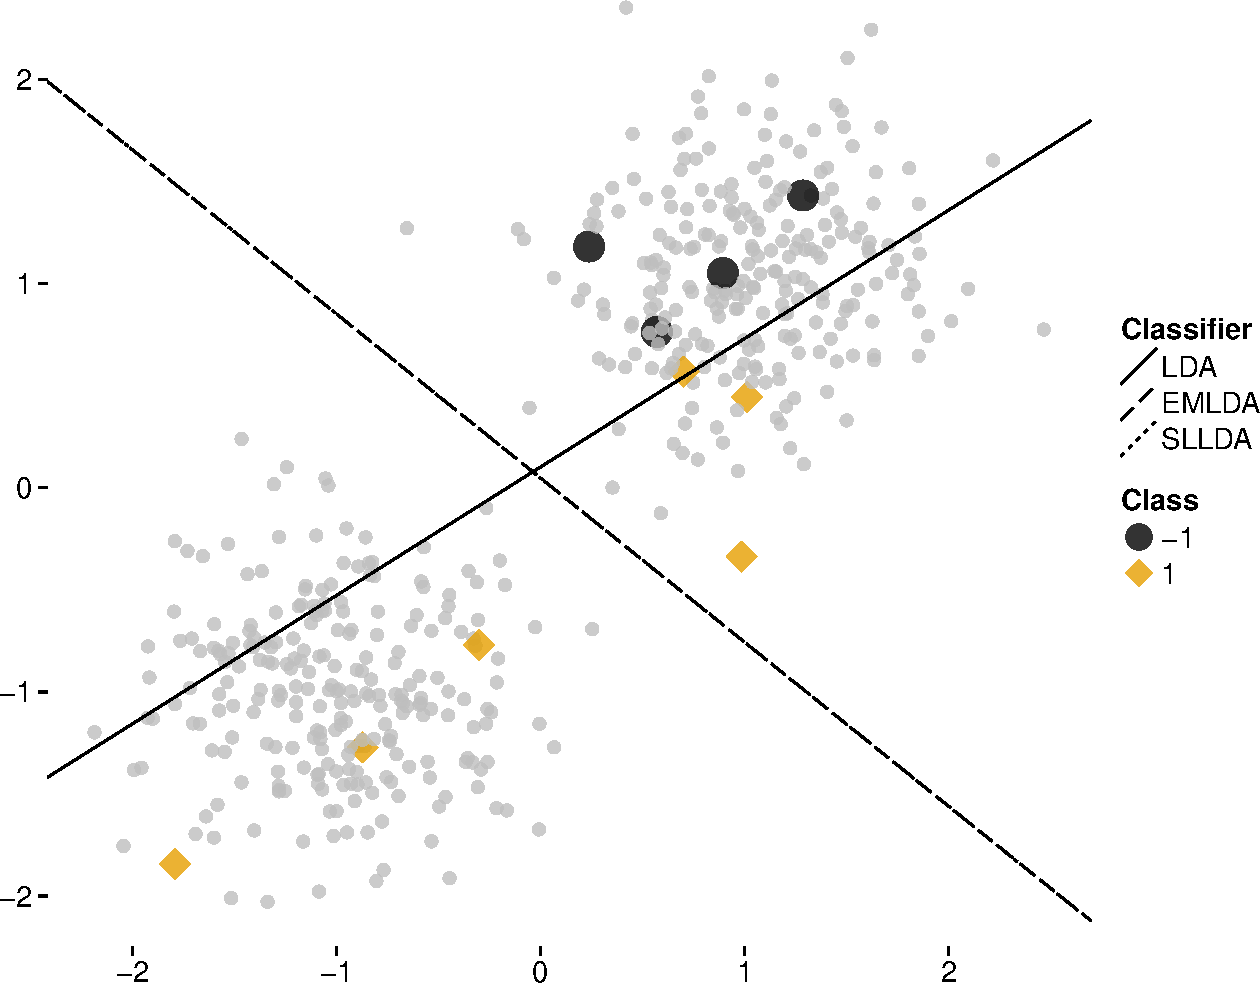
\includegraphics[width=0.99\columnwidth]{Figure1.pdf}
\caption{Self-Learning and the related Expectation Maximization type approaches work by using model predictions to impute the missing labels, after which the model is updated using these estimated labels. In this artificial dataset, self-learning and expectation-maximization versions of the linear discriminant classifier \emph{reduce} performance compared to the supervised learner.}
\end{figure}

\subsection{Low Density Separation}
\begin{figure}
\centering
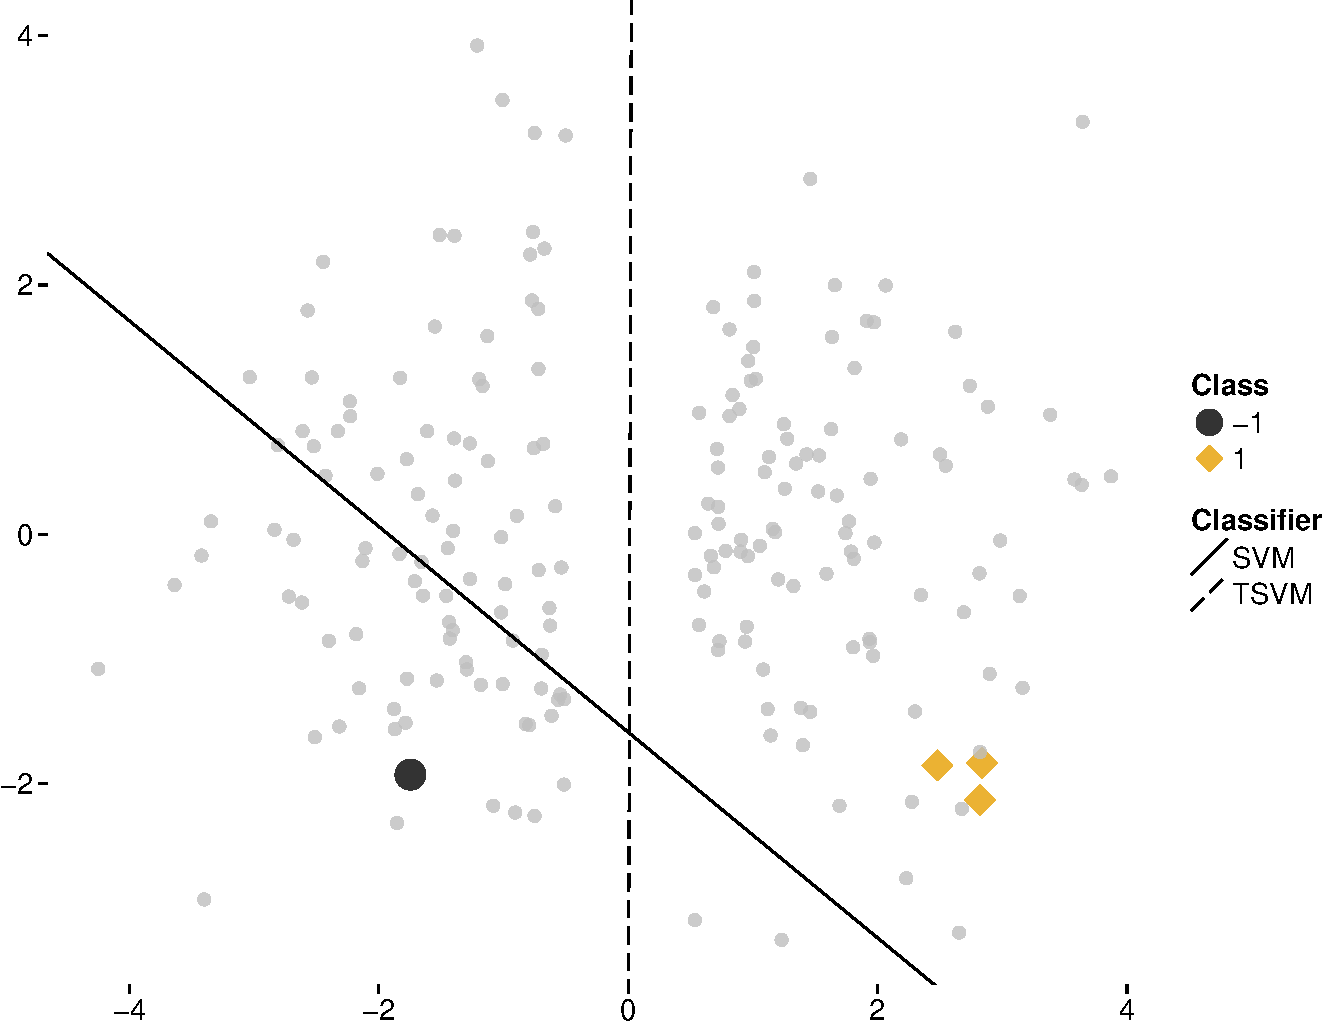
\includegraphics[width=0.99\columnwidth]{Figure2.pdf}
\caption{The Transductive SVM and related approaches nudge the decision boundary towards regions of low data density. In this artificial dataset, this assumption is useful and Transductive SVM leads to improved performance over the supervised SVM.}
\end{figure}
\vfill
\columnbreak

\section{Code Example}
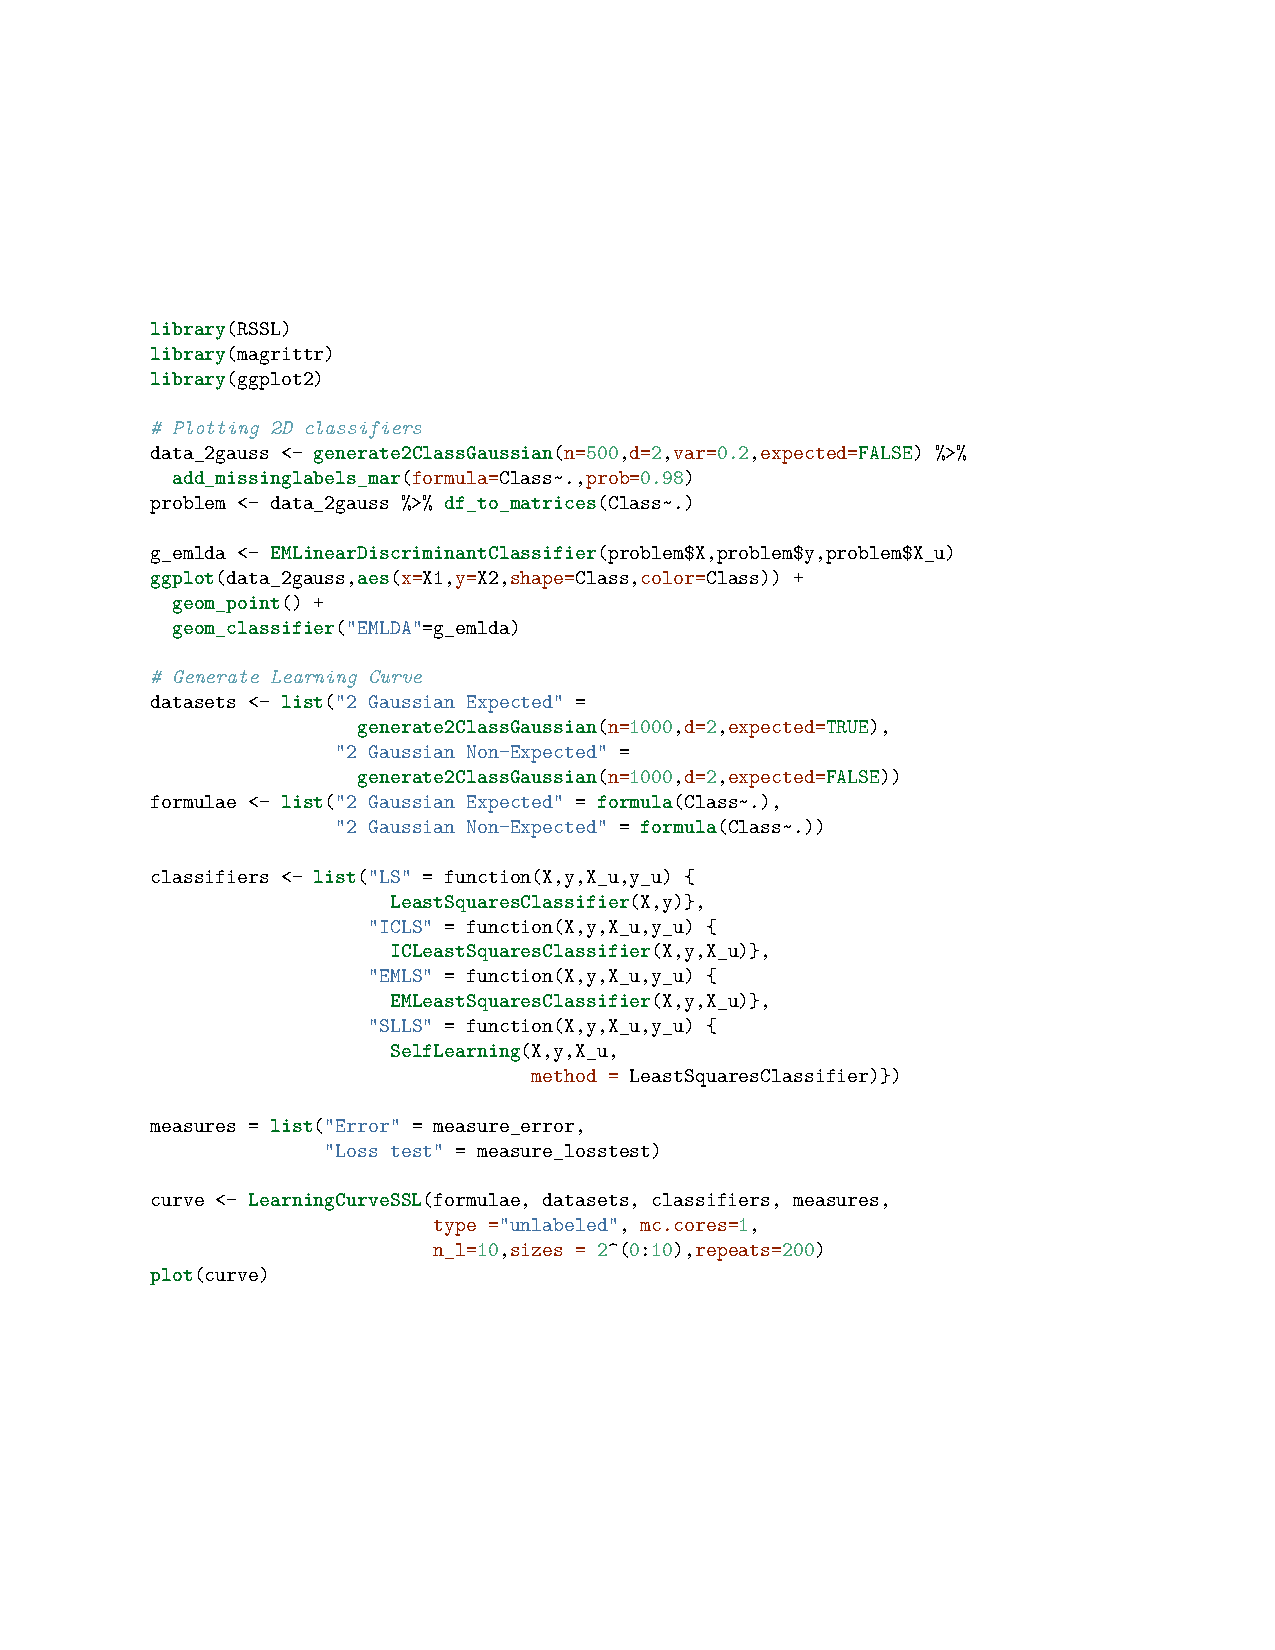
\includegraphics[width=0.90\columnwidth]{examplecode.pdf}
\vfill
\bigskip
\bigskip
\subsection{Manifold Assumption}
\begin{figure}
\centering
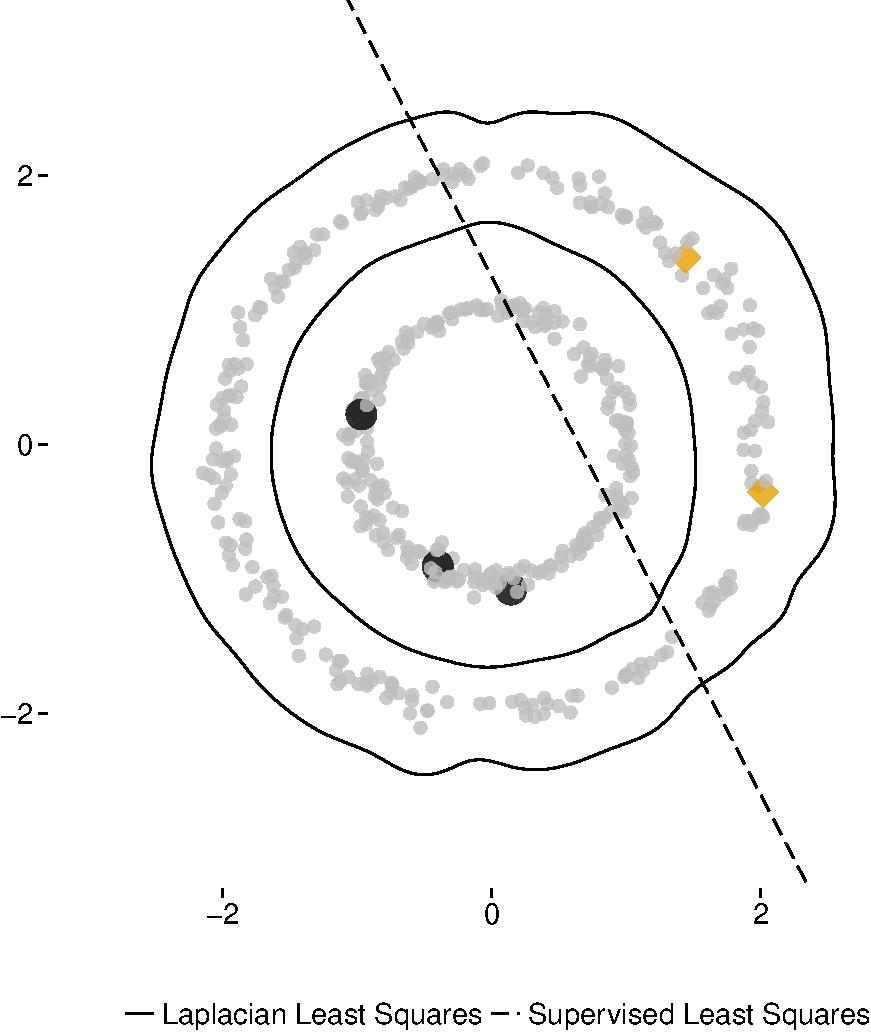
\includegraphics[width=0.70\columnwidth]{Figure3.pdf}
\caption{Assuming the labels change smoothly over the data manifolds makes it possible to "propagate" labels over the unlabeled data by ensuring its imputed label has to be similar to those objects that are close by. The Laplacian Regularized Least Squares Classifier with an RBF kernel is able to leverage this assumption to improve over the linear Least Squares Classifier.}
\end{figure}


\subsection{Robust Estimation}
\begin{figure}
\centering
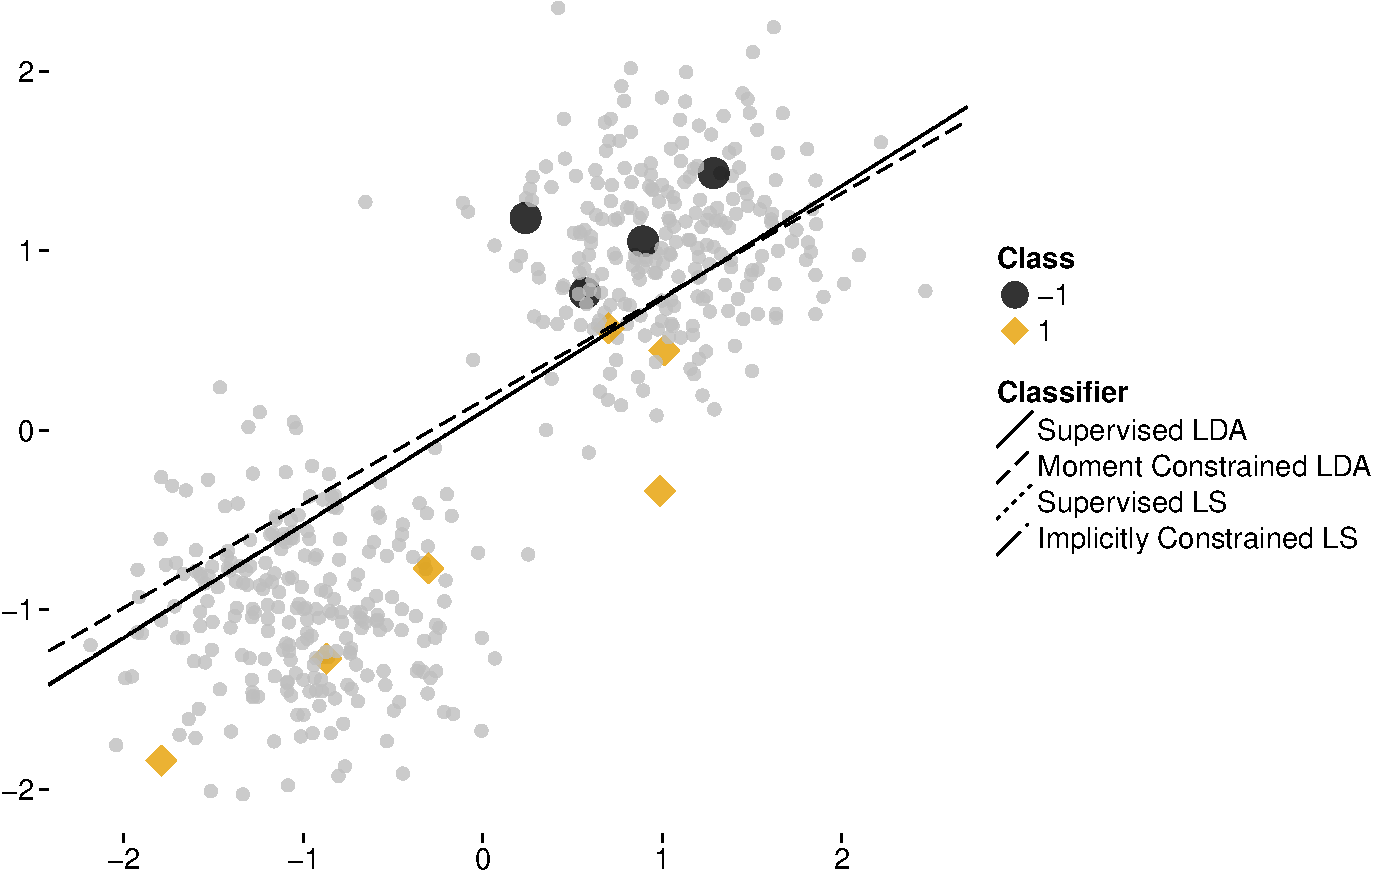
\includegraphics[width=0.99\columnwidth]{Figure4.pdf}
\caption{Compared to the first example, the goal of robust or "safe" methods is to ensure we at least do not reduce performance compared to the supervised alternative. Compare this to the self-learning methods, which are less conservative, leading to degraded performance on this dataset.}
\end{figure}


\vfill
\columnbreak

\section{Evaluation}
\subsection{Learning Curves}
\begin{figure}
\centering
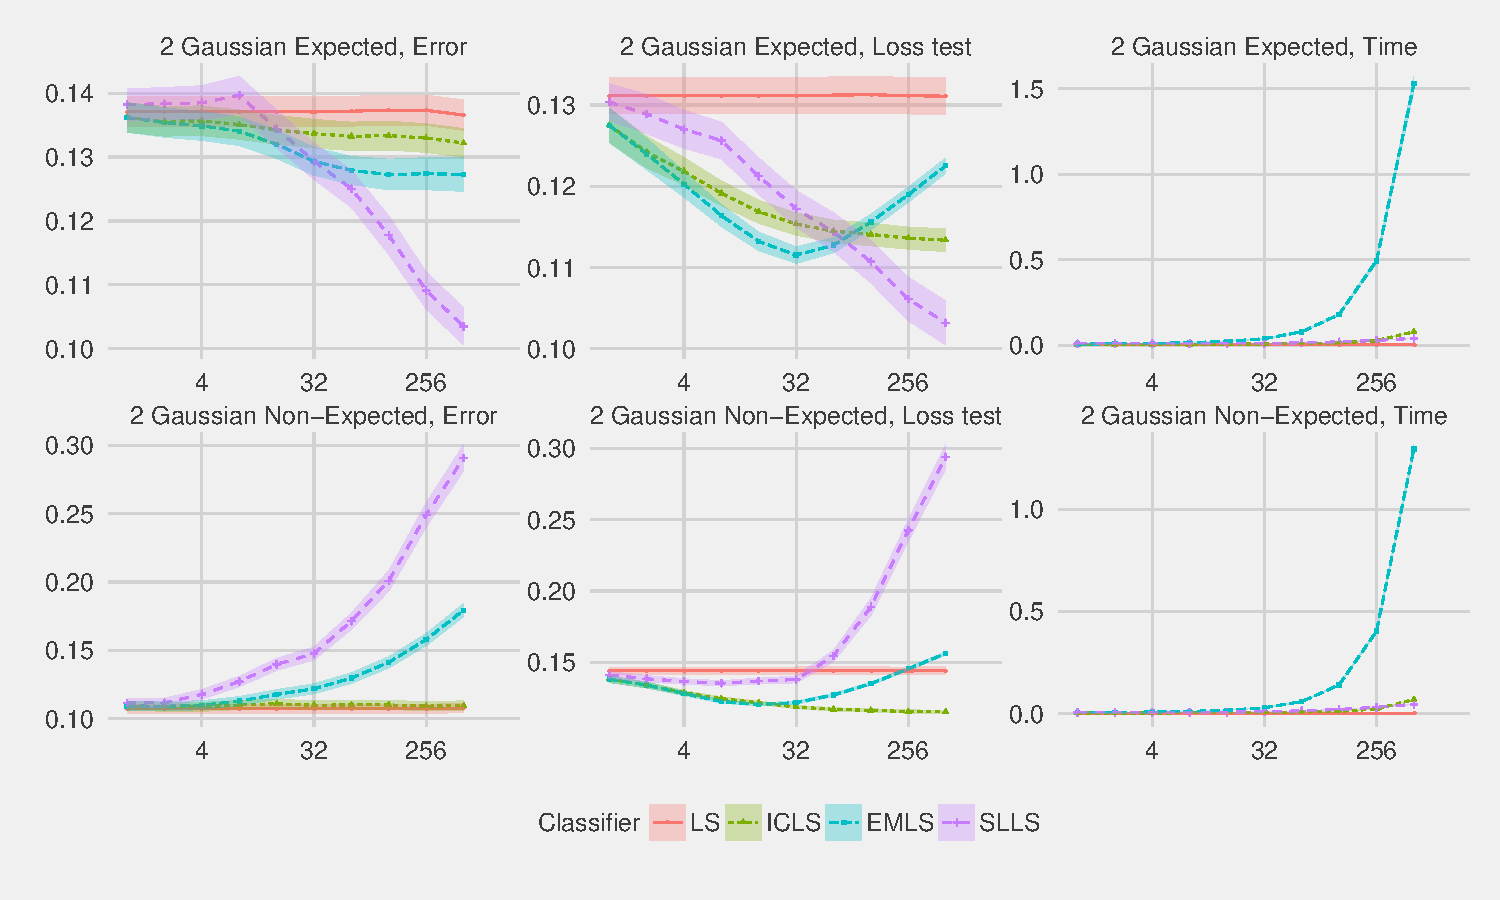
\includegraphics[width=0.98\columnwidth]{Figure5.pdf}
\caption{Example of a learning curve for the behaviour of different semi-supervised learning approaches as the number of unlabeled objects is increased, using $10$ labeled objects. The datasets are the same as the two class gaussian dataset used before when either the classes correspond to the gaussian clusters (top) or the true decision boundary crosses the classes (bottom).}
\end{figure}

\begin{figure}
\centering
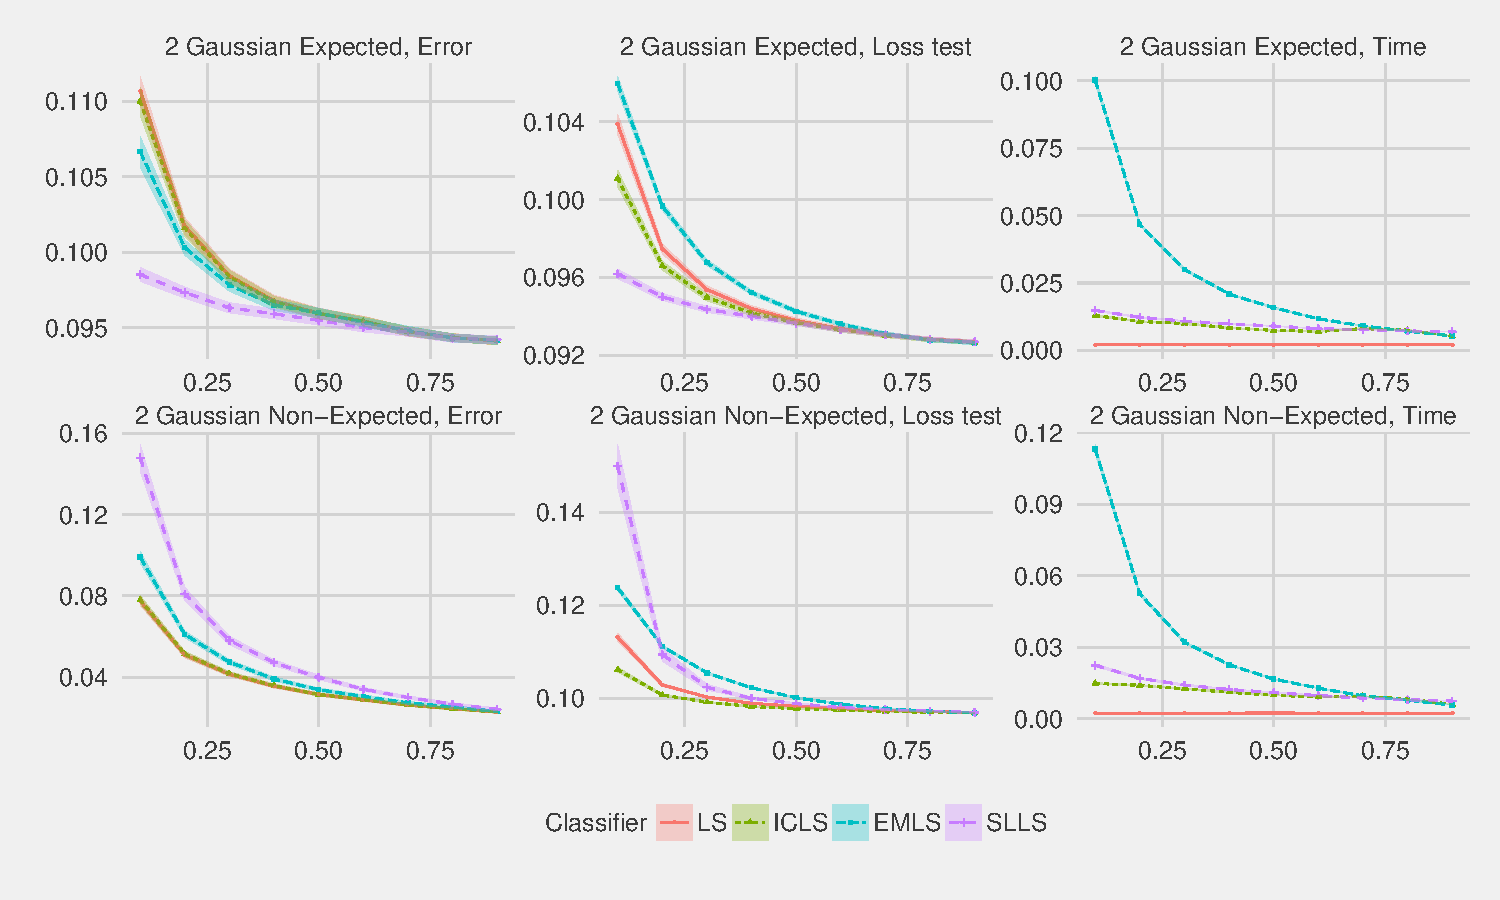
\includegraphics[width=0.98\columnwidth]{Figure6.pdf}
\caption{Similar setup to the previous figure, but now the \emph{fraction} of labeled objects is varied. The total number of objects is $200$, while $800$ objects are used for evaluating the performance.}
\end{figure}


\subsection{Cross-Validation}

\begin{table}

\resizebox{0.99\columnwidth}{!}{
\begin{tabular}{llllr}
  \hline
Dataset & Supervised \hspace{0.3cm} & Self-Learning \hspace{0.3cm} & ICLS \hspace{01.3cm} & Oracle \\ 
  \hline
 Ionosphere & 0.29 & 0.24 (1) & \textbf{0.19 (0)} & 0.13 \\ 
  Parkinsons & 0.33 & 0.29 (3) & 0.27 (0) & 0.11 \\ 
  Diabetes  & 0.32 & \underline{0.33 (16)} & \textbf{0.31 (2)} & 0.23 \\ 
  Sonar  & 0.42 & 0.37 (1) & \textbf{0.32 (1)} & 0.25 \\ 
  SPECT  & 0.42 & 0.40 (7) & \textbf{0.33 (0)} & 0.17 \\ 
  WDBC  & 0.27 & 0.17 (0) & \textbf{0.12 (0)} & 0.04 \\ 
  Digit1  & 0.41 & 0.34 (0) & \textbf{0.20 (0)} & 0.06 \\ 
  BCI  & 0.40 & 0.35 (0) & \textbf{0.28 (0)} & 0.16 \\ 
  g241d  & 0.45 & 0.39 (0) & \textbf{0.29 (0)} & 0.13 \\ 
   \hline
\end{tabular}
}
\medskip
\caption{Example of a cross-validation experiment. Indicated in $\mathbf{bold}$ is when a semi-supervised classifier has significantly lower error than the other, using a Wilcoxon signed rank test at $0.01$ significance level. A similar test is done to determine whether a semi-supervised classifier is significantly worse than the supervised classifier, indicated by \underline{underlined} values.} \label{table:cvresults}
\end{table}


\section{Discussion}
\begin{itemize}
\item What interface for the classifiers best facilitates interaction with other packages providing hyperparameter search and model selection?
\item Should we aim for replicability, calling the original implementations of the different methods, or reproducibility, by providing new implementations in R?
\end{itemize}

\end{multicols}

%==============================================================================
\end{frame}
\end{document}
